\documentclass{beamer}\usepackage[]{graphicx}\usepackage[]{color}
%% maxwidth is the original width if it is less than linewidth
%% otherwise use linewidth (to make sure the graphics do not exceed the margin)
\makeatletter
\def\maxwidth{ %
  \ifdim\Gin@nat@width>\linewidth
    \linewidth
  \else
    \Gin@nat@width
  \fi
}
\makeatother

\definecolor{fgcolor}{rgb}{0.196, 0.196, 0.196}
\newcommand{\hlnum}[1]{\textcolor[rgb]{0.063,0.58,0.627}{#1}}%
\newcommand{\hlstr}[1]{\textcolor[rgb]{0.063,0.58,0.627}{#1}}%
\newcommand{\hlcom}[1]{\textcolor[rgb]{0.588,0.588,0.588}{#1}}%
\newcommand{\hlopt}[1]{\textcolor[rgb]{0.196,0.196,0.196}{#1}}%
\newcommand{\hlstd}[1]{\textcolor[rgb]{0.196,0.196,0.196}{#1}}%
\newcommand{\hlkwa}[1]{\textcolor[rgb]{0.231,0.416,0.784}{#1}}%
\newcommand{\hlkwb}[1]{\textcolor[rgb]{0.627,0,0.314}{#1}}%
\newcommand{\hlkwc}[1]{\textcolor[rgb]{0,0.631,0.314}{#1}}%
\newcommand{\hlkwd}[1]{\textcolor[rgb]{0.78,0.227,0.412}{#1}}%
\let\hlipl\hlkwb

\usepackage{framed}
\makeatletter
\newenvironment{kframe}{%
 \def\at@end@of@kframe{}%
 \ifinner\ifhmode%
  \def\at@end@of@kframe{\end{minipage}}%
  \begin{minipage}{\columnwidth}%
 \fi\fi%
 \def\FrameCommand##1{\hskip\@totalleftmargin \hskip-\fboxsep
 \colorbox{shadecolor}{##1}\hskip-\fboxsep
     % There is no \\@totalrightmargin, so:
     \hskip-\linewidth \hskip-\@totalleftmargin \hskip\columnwidth}%
 \MakeFramed {\advance\hsize-\width
   \@totalleftmargin\z@ \linewidth\hsize
   \@setminipage}}%
 {\par\unskip\endMakeFramed%
 \at@end@of@kframe}
\makeatother

\definecolor{shadecolor}{rgb}{.97, .97, .97}
\definecolor{messagecolor}{rgb}{0, 0, 0}
\definecolor{warningcolor}{rgb}{1, 0, 1}
\definecolor{errorcolor}{rgb}{1, 0, 0}
\newenvironment{knitrout}{}{} % an empty environment to be redefined in TeX

\usepackage{alltt}

% load packages
\usepackage{tikz}
\usepackage{graphicx}
\usepackage{upquote}
\usepackage{listings}
\usepackage{hyperref}
\usepackage{color}
\usepackage{lmodern}



% define a bunch of colors
\definecolor{gray}{RGB}{110,110,110}
\definecolor{darkgray}{RGB}{100,100,100}
\definecolor{lightgray}{RGB}{200,200,200}
\definecolor{lightgrey}{RGB}{200,200,200}
\definecolor{turquoise}{RGB}{81,193,188}
\definecolor{mamey}{RGB}{255,107,107}
\definecolor{tomato}{RGB}{255,136,136}
\definecolor{mandarina}{RGB}{229,169,25}
\definecolor{lemon}{rgb}{0.81,0.95,0.29}
\definecolor{bluesky}{rgb}{0.71,0.81,0.96}
\definecolor{chiclamino}{RGB}{107,174,214}
\definecolor{violet}{RGB}{133,135,211}

\definecolor{foreground}{RGB}{81,141,193}
\definecolor{background}{RGB}{246,244,240}
\definecolor{highlight}{RGB}{229,169,25}
\definecolor{lowlight}{RGB}{200,200,200}

% setting beamer colors
\setbeamercolor{title}{fg=lightgray}
\setbeamercolor{frametitle}{fg=lightgray}
\setbeamercolor{block title}{fg=turquoise}
\setbeamercolor{structure}{fg=turquoise}
\setbeamercolor{titlelike}{fg=title}
\setbeamercolor{subtitle}{fg=turquoise}
\setbeamercolor{institute}{fg=gray}
\setbeamercolor{normal text}{fg=gray,bg=background}

\setbeamercolor{palette primary}{fg=lightgray}
\setbeamercolor{palette secondary}{fg=lightgray}
\setbeamercolor{palette tertiary}{fg=lightgray}

\setbeamerfont{itemize/enumerate subbody}{size=\footnotesize}
\setbeamerfont{itemize/enumerate subitem}{size=\footnotesize}

\hypersetup{
  colorlinks=true,
  urlcolor=tomato,
  linkcolor=lightgray
}

% commands
\newcommand{\code}[1]{\texttt{#1}}
\newcommand{\high}[1]{\textcolor{highlight}{#1}}
\newcommand{\low}[1]{\textcolor{lowlight}{#1}}
\newcommand{\highcode}[1]{\textcolor{highlight}{\texttt{#1}}}


%\usecolortheme{rose}
\setbeamertemplate{blocks}[rounded]
\setbeamertemplate{footline}[frame number] 
\setbeamertemplate{navigation symbols}{}
\setbeamertemplate{frametitle}[default][center]
\useoutertheme{infolines}  % add footlines
\setbeamersize{text margin left=25pt,text margin right=25pt}



% to remove empty brackets of \institution
\makeatletter
\setbeamertemplate{footline}
{
  \leavevmode%
  \hbox{%
  \begin{beamercolorbox}[wd=.333333\paperwidth,ht=2.25ex,dp=1ex,center]{author in head/foot}%
    \usebeamerfont{author in head/foot}\insertshortauthor%~~\beamer@ifempty{\insertshortinstitute}{}{(\insertshortinstitute)}
  \end{beamercolorbox}%
  \begin{beamercolorbox}[wd=.333333\paperwidth,ht=2.25ex,dp=1ex,center]{title in head/foot}%
    \usebeamerfont{title in head/foot}\insertshorttitle
  \end{beamercolorbox}%
  \begin{beamercolorbox}[wd=.333333\paperwidth,ht=2.25ex,dp=1ex,right]{date in head/foot}%
    \usebeamerfont{date in head/foot}\insertshortdate{}\hspace*{2em}
    \insertframenumber{} / \inserttotalframenumber\hspace*{2ex} 
  \end{beamercolorbox}}%
  \vskip0pt%
}
\makeatother



\title[Getting data from the web with R]{\LARGE Getting Data from the Web with R} 
\subtitle[Web Data in R]{\large Part 5: Handling JSON data}
\author[gastonsanchez.com]{
 \textcolor{gray}{\textbf{G}aston \textbf{S}anchez}
}
\institute[]{\scriptsize \textcolor{lightgray}{April-May 2014}}
\date[CC BY-SA-NC 4.0]{
 \textcolor{lightgray}{\tiny{Content licensed under 
 \href{http://creativecommons.org/licenses/by-nc-sa/4.0/}{CC BY-NC-SA 4.0}}}
}
\IfFileExists{upquote.sty}{\usepackage{upquote}}{}
\begin{document}



%--- the titlepage frame -------------------------%

\begin{frame}[plain]
 \titlepage
\end{frame}

%------------------------------------------------

{ % all template changes are local to this group.
    \setbeamertemplate{navigation symbols}{}
    \begin{frame}[plain]
        \begin{tikzpicture}[remember picture,overlay]
            \node[at=(current page.center)] {
                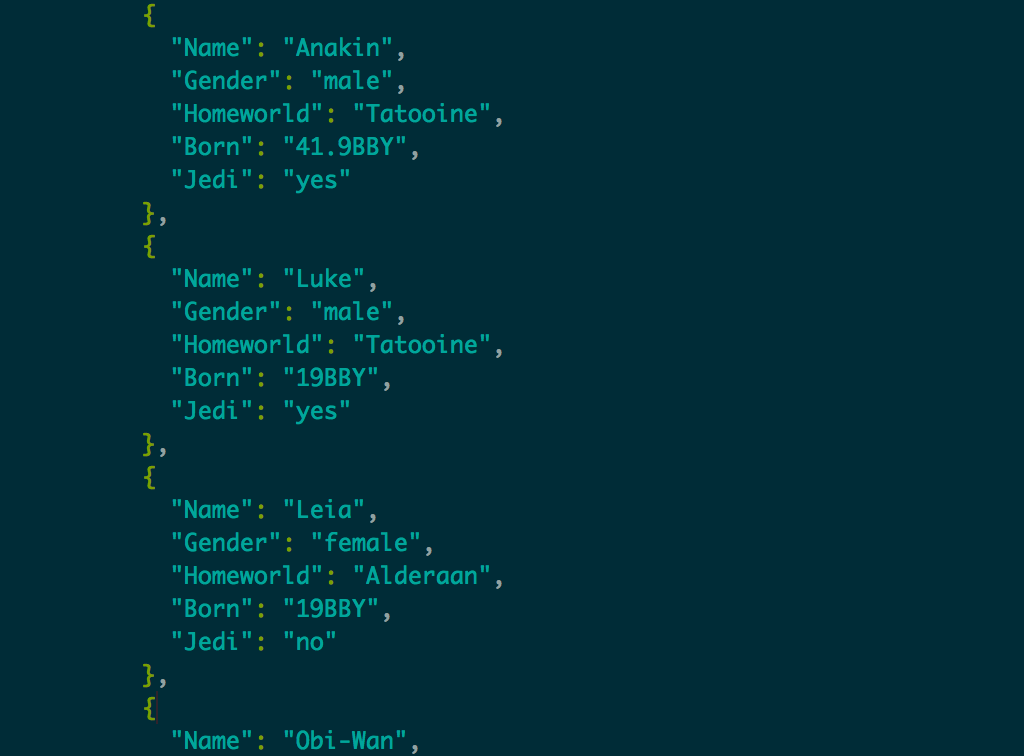
\includegraphics[width=\paperwidth]{images/json_cover.png}
            };
        \end{tikzpicture}
     \end{frame}
}

%------------------------------------------------

\begin{frame}[fragile]
\frametitle{Readme}

\begin{block}{\scriptsize License:}
\tiny
 \begin{itemize}
  \item[] Creative Commons Attribution-NonCommercial-ShareAlike 4.0 International License \\ 
  \url{http://creativecommons.org/licenses/by-nc-sa/4.0/}{}
 \end{itemize}
\end{block}

\begin{block}{\scriptsize You are free to:}
\tiny
 \begin{itemize}
  \item[] \textcolor{darkgray}{\textbf{Share}} --- \textcolor{gray}{copy and redistribute the material}
  \item[] \textcolor{darkgray}{\textbf{Adapt}} --- \textcolor{gray}{rebuild and transform the material}
 \end{itemize}
\end{block}

\vspace{2mm}
\begin{block}{\scriptsize Under the following conditions:}
\tiny
\begin{itemize}
 \item[] \textcolor{darkgray}{\textbf{Attribution}} --- \textcolor{gray}{You must give appropriate credit, provide a link to the license, and indicate if changes were made.}
 \item[] \textcolor{darkgray}{\textbf{NonCommercial}} --- \textcolor{gray}{You may not use this work for commercial purposes.}
 \item[] \textcolor{darkgray}{\textbf{Share Alike}} --- \textcolor{gray}{If you remix, transform, or build upon this 
 work, you must distribute your contributions under the same license to this one.}
\end{itemize}
\end{block}

\end{frame}

%------------------------------------------------

\begin{frame}
\frametitle{Lectures Menu}

\begin{columns}[t]
\begin{column}{0.1\textwidth}
%--- empty space ---%
\end{column}
\begin{column}{0.8\textwidth}
 \begin{block}{Slide Decks}
  \begin{enumerate}
   \item \textcolor{lightgray}{Introduction}
   \item \textcolor{lightgray}{Reading files from the Web}
   \item \textcolor{lightgray}{Basics of XML and HTML}
   \item \textcolor{lightgray}{Parsing XML / HTML content}
   \item \textbf{Handling JSON data}
   \item \textcolor{lightgray}{HTTP Basics and the RCurl Package}
   \item \textcolor{lightgray}{Getting data via Web Forms}
   \item \textcolor{lightgray}{Getting data via Web APIs}
  \end{enumerate}
 \end{block}
\end{column}
\begin{column}{0.1\textwidth}
%--- empty space ---%
\end{column}
\end{columns}

\end{frame}

%------------------------------------------------

\begin{frame}
 \begin{center}
  \Huge{\textcolor{mandarina}{JSON Data}}
 \end{center}
\end{frame}

%------------------------------------------------

\begin{frame}
\frametitle{Goal}

\begin{columns}[t]
\begin{column}{0.1\textwidth}
%--- empty space ---%
\end{column}
\begin{column}{0.8\textwidth}

\begin{block}{JSON}
The goal of these slides is to provide an introduction for \textbf{handling JSON data in R}
\end{block}

\end{column}
\begin{column}{0.1\textwidth}
%--- empty space ---%
\end{column}
\end{columns}

\end{frame}

%------------------------------------------------

\begin{frame}
\frametitle{Synopsis}

\begin{columns}[t]
\begin{column}{0.1\textwidth}
%--- empty space ---%
\end{column}
\begin{column}{0.8\textwidth}

\begin{block}{In a nutshell}
We'll cover the following topics:
\begin{itemize}
 \item JSON Basics
 \item R packages for JSON data
 \item Reading JSON data from the Web
\end{itemize}
\end{block}

\end{column}
\begin{column}{0.1\textwidth}
%--- empty space ---%
\end{column}
\end{columns}

\end{frame}

%------------------------------------------------

\begin{frame}
\frametitle{Some References}

\begin{itemize}
 \item XML and Web Technlogies for Data Sciences with R \\
 \low{by Deb Nolan and Duncan Temple Lang}
 \item Introducing JSON \\
 {\scriptsize \url{http://www.json.org/}}
 \item R package RJSONIO \\
 {\scriptsize \url{http://cran.r-project.org/web/packages/RJSONIO/index.html}}
 \item R package jsonlite \\
{\scriptsize \url{http://cran.r-project.org/web/packages/jsonlite/vignettes/json-mapping.pdf}}
 \item R package rjson \\
{\scriptsize \url{http://cran.r-project.org/web/packages/rjson/index.html}}
\end{itemize}

\end{frame}

%------------------------------------------------

\begin{frame}
 \begin{center}
  \Huge{\textcolor{mandarina}{JSON Basics}}
 \end{center}
\end{frame}

%------------------------------------------------

\begin{frame}
\frametitle{Basics First}

\begin{columns}[t]
\begin{column}{0.1\textwidth}
%--- empty space ---%
\end{column}
\begin{column}{0.7\textwidth}

\begin{block}{Fundamentals}
JSON stands for \textbf{JavaScript Object Notation} \\
and it is a format for representing data
 \begin{itemize}
  \item general purpose format
  \item lightweight format
  \item widely popular
  \item fairly simple
 \end{itemize}
\end{block}

\end{column}
\begin{column}{0.1\textwidth}
%--- empty space ---%
\end{column}
\end{columns}

\end{frame}

%------------------------------------------------

\begin{frame}
\frametitle{Basics First}

\begin{block}{Why should we care?}
When working with data from the Web, we'll inevitably find some JSON data
\begin{itemize}
 \item JSON can be used directly in JavaScript code for Web pages
 \item many Web APIs provide data in JSON format
 \item R has packages designed to handle JSON data
\end{itemize}
\end{block}

\end{frame}

%------------------------------------------------

\begin{frame}
 \begin{center}
  \Huge{\textcolor{mandarina}{Understanding JSON}}
 \end{center}
\end{frame}

%------------------------------------------------

\begin{frame}
\frametitle{Understanding JSON}

\begin{columns}[t]
\begin{column}{0.3\textwidth}
 \begin{block}{JSON Data Types}
  \begin{itemize}
   \item[] \highcode{null}
   \item[] \highcode{true}
   \item[] \highcode{false}
   \item[] \highcode{number}
   \item[] \highcode{string}
  \end{itemize}
 \end{block}
\end{column}

\begin{column}{0.4\textwidth}
 \begin{block}{JSON Data Containers}
  \begin{itemize}
   \item[] square brackets \highcode{[ ]}
   \item[] curly brackets \highcode{\{ \}}
  \end{itemize}
 \end{block}
\end{column}
\end{columns}

\end{frame}

%------------------------------------------------

\begin{frame}
\frametitle{JSON Arrays}

\begin{block}{Unnamed Arrays}
Square brackets \highcode{[ ]} are used for \textbf{ordered unnamed arrays}
\begin{itemize}
 \item \code{ [ 1, 2, 3, ... ] }
 \item \code{ [ true, true, false, ... ] }
\end{itemize}
\end{block}

\begin{block}{Named Arrays}
Curly brackets \highcode{\{ \}} are used for \textbf{named arrays}
\begin{itemize}
 \item \code{ \{ "dollars" : 5, "euros" : 20, ... \} }
 \item \code{ \{ "city" : "Berkeley", "state" : "CA", ... \} }
\end{itemize}
\end{block}

\end{frame}

%------------------------------------------------

\begin{frame}[fragile]
\frametitle{JSON Arrays}

Containers can be nested

\begin{columns}[t]
\begin{column}{0.5\textwidth}
\begin{block}{Example A}
{\footnotesize
\begin{verbatim}
{
    "name": ["X", "Y", "Z"],
    "grams": [300, 200, 500], 
    "qty": [4, 5, null],
    "new": [true, false, true],
}
\end{verbatim}
}
\end{block}
\end{column}

\begin{column}{0.5\textwidth}
\begin{block}{Example B}
{\footnotesize
\begin{verbatim}
[
    { "name": "X", 
      "grams": 300,
      "qty": 4,
      "new": true },
    { "name": "Y",
      "grams": 200,
      "qty": 5,
      "new": false },
    { "name": "Z",
      "grams": 500, 
      "qty": null,
      "new": true}
]
\end{verbatim}
}
\end{block}
\end{column}
\end{columns}

\end{frame}

%------------------------------------------------

\begin{frame}[fragile]
\frametitle{Data Table Toy Example}

\begin{center}
\textcolor{turquoise}{Imagine we have some data}

\bigskip
\begin{tabular}{l l l l l}
  \hline
  Name & Gender & Homeland & Born & Jedi \\
  \hline
  Anakin & male & Tatooine & 41.9BBY & yes \\  
  Amidala & female & Naboo & 46BBY & no \\
  Luke & male & Tatooine & 19BBY & yes \\
  Leia & female & Alderaan & 19BBY & no \\
  Obi-Wan & male & Stewjon & 57BBY & yes \\
  Han & male & Corellia & 29BBY & no \\
  Palpatine & male & Naboo & 82BBY & no \\
  R2-D2 & unknown & Naboo & 33BBY & no \\
  \hline
 \end{tabular}
\end{center}

There are several ways to represent this data in JSON format

\end{frame}

%------------------------------------------------

\begin{frame}[fragile]
\frametitle{One way to represent data}

{\footnotesize
\begin{verbatim}
    [
        {
         "Name": "Anakin",
         "Gender": "male", 
         "Homeworld": "Tatooine",
         "Born": "41.9BBY",
         "Jedi": "yes"
        },
        ...
        {
         "Name": "R2-D2",
         "Gender": "unknown",
         "Homeworld": "Naboo",
         "Born": "33BBY",
         "Jedi": "no"
        },
    ]
\end{verbatim}
}
\end{frame}

%------------------------------------------------

\begin{frame}[fragile]
\frametitle{Another way to represent data}

{\footnotesize
\begin{verbatim}
{
  "Name": [ "Anakin", "Amidala", "Luke", ... , "R2-D2" ],
  "Gender": [ "male", "female", "male", ... , "unknown" ],
  "Homeworld": [ "Tatooine", "Naboo", "Tatooine", ... , "Naboo" ],
  "Born": [ "41.9BBY", "46BBY", "19BBY", ... , "33BBY" ],
  "Jedi": [ "yes", "no", "yes", ... , "no" ] 
}

\end{verbatim}
}
\end{frame}

%------------------------------------------------

\begin{frame}
 \begin{center}
  \Huge{\textcolor{mandarina}{JSON R packages}}
 \end{center}
\end{frame}

%------------------------------------------------

\begin{frame}
\frametitle{R packages}

\begin{block}{R packages for JSON}
R has 3 packages for working with JSON data

\begin{itemize}
 \item \highcode{"RJSONIO"} by Duncan Temple Lang
 \item \highcode{"rjson"} by Alex Couture-Beil
 \item \highcode{"jsonlite"} by Jeroen Ooms, Duncan Temple Lang, Jonathan Wallace
\end{itemize}
\end{block}

All packages provide 2 main functions ---\highcode{toJSON()} and \highcode{fromJSON()}--- that allow conversion \textbf{to} and \textbf{from} data in JSON format, respectively. \\
\low{We'll focus on the functions from \code{"RJSONIO"}}

\end{frame}

%------------------------------------------------

\begin{frame}[fragile]
\frametitle{R package RJSONIO}

\begin{block}{R package \code{"RJSONIO"}}
If you don't have \code{"RJSONIO"} you'll have to install it:
\begin{knitrout}\small
\definecolor{shadecolor}{rgb}{1, 1, 1}\color{fgcolor}\begin{kframe}
\begin{alltt}
\hlcom{# install RJSONIO}
\hlkwd{install.packages}\hlstd{(}\hlstr{"RJSONIO"}\hlstd{,} \hlkwc{dependencies} \hlstd{=} \hlnum{TRUE}\hlstd{)}
\end{alltt}
\end{kframe}
\end{knitrout}
\end{block}

\end{frame}

%------------------------------------------------

\begin{frame}[fragile]
\frametitle{R package RJSONIO}

\begin{block}{Main functions}
There are 2 primary functions in \code{"RJSONIO"}
\begin{itemize}
 \item \highcode{toJSON()} converts an R object to a string in JSON
 \item \highcode{fromJSON()} converts JSON content to R objects
\end{itemize}
\end{block}

\end{frame}

%------------------------------------------------

\begin{frame}[fragile]
\frametitle{\code{toJSON()}}

\begin{block}{Function \code{toJSON()}}
\begin{verbatim}
toJSON(x, container = isContainer(x, asIs, .level), 
       collapse = "\n", ...)
\end{verbatim}

\begin{itemize}
 \item \highcode{x} the R object to be converted to JSON format
 \item \highcode{container} whether to treat the object as a vector/container or a scalar 
 \item \highcode{collapse} string used as separator when combining the individual lines of the generated JSON content
 \item \highcode{...} additional arguments controlling the JSON formatting
\end{itemize}
\end{block}

\end{frame}

%------------------------------------------------

\begin{frame}[fragile]
\frametitle{\code{fromJSON()}}

\begin{block}{Function \code{fromJSON()}}
\begin{verbatim}
fromJSON(content, handler = NULL, default.size = 100,
         depth = 150L, allowComments = TRUE, ...)
\end{verbatim}

\begin{itemize}
 \item \highcode{content} the JSON content: either a file name or a character string
 \item \highcode{handler} R object responsible for processing each individual token/element
 \item \highcode{deafult.size} size to use for arrays and objects in an effort to avoid reallocating each time we add a new element.
 \item \highcode{depth} maximum number of nested JSON levels
 \item \highcode{allowComments} whether to allow C-style comments within the JSON content
 \item \highcode{...} additional parameters
\end{itemize}
\end{block}

\end{frame}

%------------------------------------------------

\begin{frame}[fragile]
\frametitle{Data Table Toy Example}

\begin{center}
\textcolor{turquoise}{Imagine we have some tabular data}
\end{center}

\begin{center}
 \begin{tabular}{l l l l l}
  \hline
  Name & Gender & Homeland & Born & Jedi \\
  \hline
  Anakin & male & Tatooine & 41.9BBY & yes \\  
  Amidala & female & Naboo & 46BBY & no \\
  Luke & male & Tatooine & 19BBY & yes \\
  Leia & female & Alderaan & 19BBY & no \\
  Obi-Wan & male & Stewjon & 57BBY & yes \\
  Han & male & Corellia & 29BBY & no \\
  Palpatine & male & Naboo & 82BBY & no \\
  R2-D2 & unknown & Naboo & 33BBY & no \\
  \hline
 \end{tabular}
\end{center}

\end{frame}

%------------------------------------------------

\begin{frame}[fragile]
\frametitle{R Data Frame}

\begin{knitrout}\tiny
\definecolor{shadecolor}{rgb}{1, 1, 1}\color{fgcolor}\begin{kframe}
\begin{alltt}
\hlcom{# toy data}
\hlstd{sw_data} \hlkwb{=} \hlkwd{rbind}\hlstd{(}
  \hlkwd{c}\hlstd{(}\hlstr{"Anakin"}\hlstd{,} \hlstr{"male"}\hlstd{,} \hlstr{"Tatooine"}\hlstd{,} \hlstr{"41.9BBY"}\hlstd{,}  \hlstr{"yes"}\hlstd{),}
  \hlkwd{c}\hlstd{(}\hlstr{"Amidala"}\hlstd{,} \hlstr{"female"}\hlstd{,} \hlstr{"Naboo"}\hlstd{,} \hlstr{"46BBY"}\hlstd{,} \hlstr{"no"}\hlstd{),}
  \hlkwd{c}\hlstd{(}\hlstr{"Luke"}\hlstd{,} \hlstr{"male"}\hlstd{,} \hlstr{"Tatooine"}\hlstd{,} \hlstr{"19BBY"}\hlstd{,} \hlstr{"yes"}\hlstd{),}
  \hlkwd{c}\hlstd{(}\hlstr{"Leia"}\hlstd{,} \hlstr{"female"}\hlstd{,} \hlstr{"Alderaan"}\hlstd{,} \hlstr{"19BBY"}\hlstd{,} \hlstr{"no"}\hlstd{),}
  \hlkwd{c}\hlstd{(}\hlstr{"Obi-Wan"}\hlstd{,}  \hlstr{"male"}\hlstd{,} \hlstr{"Stewjon"}\hlstd{,} \hlstr{"57BBY"}\hlstd{,} \hlstr{"yes"}\hlstd{),}
  \hlkwd{c}\hlstd{(}\hlstr{"Han"}\hlstd{,} \hlstr{"male"}\hlstd{,} \hlstr{"Corellia"}\hlstd{,} \hlstr{"29BBY"}\hlstd{,} \hlstr{"no"}\hlstd{),}
  \hlkwd{c}\hlstd{(}\hlstr{"Palpatine"}\hlstd{,} \hlstr{"male"}\hlstd{,} \hlstr{"Naboo"}\hlstd{,} \hlstr{"82BBY"}\hlstd{,} \hlstr{"no"}\hlstd{),}
  \hlkwd{c}\hlstd{(}\hlstr{"R2-D2"}\hlstd{,} \hlstr{"unknown"}\hlstd{,} \hlstr{"Naboo"}\hlstd{,} \hlstr{"33BBY"}\hlstd{,} \hlstr{"no"}\hlstd{))}

\hlcom{# convert to data.frame and add column names}
\hlstd{swdf} \hlkwb{=} \hlkwd{data.frame}\hlstd{(sw_data)}
\hlkwd{names}\hlstd{(swdf)} \hlkwb{=} \hlkwd{c}\hlstd{(}\hlstr{"Name"}\hlstd{,} \hlstr{"Gender"}\hlstd{,} \hlstr{"Homeworld"}\hlstd{,} \hlstr{"Born"}\hlstd{,} \hlstr{"Jedi"}\hlstd{)}
\hlstd{swdf}
\end{alltt}
\begin{verbatim}
##        Name  Gender Homeworld    Born Jedi
## 1    Anakin    male  Tatooine 41.9BBY  yes
## 2   Amidala  female     Naboo   46BBY   no
## 3      Luke    male  Tatooine   19BBY  yes
## 4      Leia  female  Alderaan   19BBY   no
## 5   Obi-Wan    male   Stewjon   57BBY  yes
## 6       Han    male  Corellia   29BBY   no
## 7 Palpatine    male     Naboo   82BBY   no
## 8     R2-D2 unknown     Naboo   33BBY   no
\end{verbatim}
\end{kframe}
\end{knitrout}

\end{frame}

%------------------------------------------------

\begin{frame}[fragile]
\frametitle{From R to JSON}

\begin{knitrout}\tiny
\definecolor{shadecolor}{rgb}{1, 1, 1}\color{fgcolor}\begin{kframe}
\begin{alltt}
\hlcom{# load RJSONIO}
\hlkwd{library}\hlstd{(RJSONIO)}

\hlcom{# convert R data.frame to JSON}
\hlstd{sw_json} \hlkwb{=} \hlkwd{toJSON}\hlstd{(swdf)}

\hlcom{# what class?}
\hlkwd{class}\hlstd{(sw_json)}
\end{alltt}
\begin{verbatim}
## [1] "character"
\end{verbatim}
\begin{alltt}
\hlcom{# display JSON format}
\hlkwd{cat}\hlstd{(sw_json)}
\end{alltt}
\begin{verbatim}
## {
##  "Name": [ "Anakin", "Amidala", "Luke", "Leia", "Obi-Wan", "Han", "Palpatine", "R2-D2" ],
## "Gender": [ "male", "female", "male", "female", "male", "male", "male", "unknown" ],
## "Homeworld": [ "Tatooine", "Naboo", "Tatooine", "Alderaan", "Stewjon", "Corellia", "Naboo", "Naboo" ],
## "Born": [ "41.9BBY", "46BBY", "19BBY", "19BBY", "57BBY", "29BBY", "82BBY", "33BBY" ],
## "Jedi": [ "yes", "no", "yes", "no", "yes", "no", "no", "no" ] 
## }
\end{verbatim}
\end{kframe}
\end{knitrout}

\end{frame}

%------------------------------------------------

\begin{frame}[fragile]
\frametitle{From JSON to R}

\begin{knitrout}\tiny
\definecolor{shadecolor}{rgb}{1, 1, 1}\color{fgcolor}\begin{kframe}
\begin{alltt}
\hlcom{# convert JSON string to R list}
\hlstd{sw_R} \hlkwb{=} \hlkwd{fromJSON}\hlstd{(sw_json)}

\hlcom{# what class?}
\hlkwd{class}\hlstd{(sw_R)}
\end{alltt}
\begin{verbatim}
## [1] "list"
\end{verbatim}
\begin{alltt}
\hlcom{# display JSON format}
\hlstd{sw_R}
\end{alltt}
\begin{verbatim}
## $Name
## [1] "Anakin"    "Amidala"   "Luke"      "Leia"      "Obi-Wan"   "Han"      
## [7] "Palpatine" "R2-D2"    
## 
## $Gender
## [1] "male"    "female"  "male"    "female"  "male"    "male"    "male"   
## [8] "unknown"
## 
## $Homeworld
## [1] "Tatooine" "Naboo"    "Tatooine" "Alderaan" "Stewjon"  "Corellia"
## [7] "Naboo"    "Naboo"   
## 
## $Born
## [1] "41.9BBY" "46BBY"   "19BBY"   "19BBY"   "57BBY"   "29BBY"   "82BBY"  
## [8] "33BBY"  
## 
## $Jedi
## [1] "yes" "no"  "yes" "no"  "yes" "no"  "no"  "no"
\end{verbatim}
\end{kframe}
\end{knitrout}

\end{frame}

%------------------------------------------------

\begin{frame}
 \begin{center}
  \Huge{\textcolor{mandarina}{Reading JSON Data}}
 \end{center}
\end{frame}

%------------------------------------------------

\begin{frame}
\frametitle{JSON Data from the Web}

\begin{block}{How do we read JSON data from the Web?}
We read JSON data in several ways. One way is to pass the url directly to \code{fromJSON()}. Another way is by passing \code{fromJSON()} the name of the file with the JSON content as a single string.
\end{block}

\end{frame}

%------------------------------------------------

\begin{frame}
\frametitle{File: miserables.js}

We'll read the \textit{miserables} dataset from: \\
\url{http://mbostock.github.io/protovis/ex/miserables.js}

\begin{center}
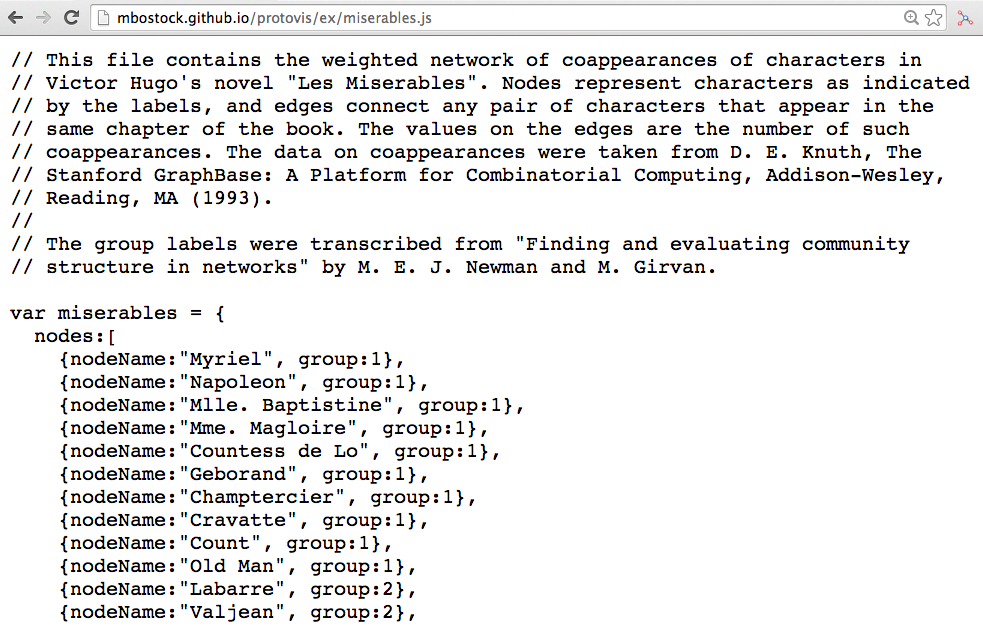
\includegraphics[width=8cm]{images/miserables_js.png}
\end{center}

\end{frame}

%------------------------------------------------

\begin{frame}
\frametitle{Reading Issues}

\begin{block}{Houston we have a problem ...}
The data is in a file that contains several javascript comments and some other javascript notation.

\bigskip
Unfortunately, we cannot use any of the \code{fromJSON()} functions directly on this type of content.

\bigskip
Instead, we need to read the content as text, get rid of the comments, and change some characters before using \code{fromJSON()}
\end{block}

\end{frame}

%------------------------------------------------

\begin{frame}[fragile]
\frametitle{Reading \code{miserables.js}}

\begin{knitrout}\tiny
\definecolor{shadecolor}{rgb}{1, 1, 1}\color{fgcolor}\begin{kframe}
\begin{alltt}
\hlcom{# load RJSONIO and jsonlite}
\hlkwd{library}\hlstd{(RJSONIO)}
\hlkwd{library}\hlstd{(jsonlite)}

\hlcom{# url with JSON content}
\hlstd{miser} \hlkwb{=} \hlstr{"http://mbostock.github.io/protovis/ex/miserables.js"}

\hlcom{# import content as text (character vector)}
\hlstd{miserables} \hlkwb{=} \hlkwd{readLines}\hlstd{(miser)}

\hlcom{# eliminate first 11 lines (containing comments)}
\hlstd{miserables} \hlkwb{=} \hlstd{miserables[}\hlopt{-}\hlkwd{c}\hlstd{(}\hlnum{1}\hlopt{:}\hlnum{11}\hlstd{)]}
\end{alltt}
\end{kframe}
\end{knitrout}



Now check the first and the last lines:

\begin{knitrout}\tiny
\definecolor{shadecolor}{rgb}{1, 1, 1}\color{fgcolor}\begin{kframe}
\begin{alltt}
\hlcom{# first line}
\hlstd{miserables[}\hlnum{1}\hlstd{]}
\end{alltt}
\begin{verbatim}
## [1] "var miserables = {"
\end{verbatim}
\begin{alltt}
\hlcom{# last line}
\hlstd{miserables[}\hlkwd{length}\hlstd{(miserables)]}
\end{alltt}
\begin{verbatim}
## [1] "};"
\end{verbatim}
\end{kframe}
\end{knitrout}

\end{frame}

%------------------------------------------------

\begin{frame}[fragile]
\frametitle{Preparing JSON content}

We need to modify the first and last lines so they don't contain non-JSON javascript notation

\begin{knitrout}\tiny
\definecolor{shadecolor}{rgb}{1, 1, 1}\color{fgcolor}\begin{kframe}
\begin{alltt}
\hlcom{# open curly bracket in first line}
\hlstd{miserables[}\hlnum{1}\hlstd{]} \hlkwb{=} \hlstr{"\{"}

\hlcom{# closing curly bracket in last line}
\hlstd{miserables[}\hlkwd{length}\hlstd{(miserables)]} \hlkwb{=} \hlstr{"\}"}
\end{alltt}
\end{kframe}
\end{knitrout}

Now we must concatenate all the content into a single string:

\begin{knitrout}\tiny
\definecolor{shadecolor}{rgb}{1, 1, 1}\color{fgcolor}\begin{kframe}
\begin{alltt}
\hlcom{# JSON content in one single string}
\hlstd{miserables_str} \hlkwb{=} \hlkwd{paste}\hlstd{(miserables,} \hlkwc{collapse} \hlstd{=} \hlstr{""}\hlstd{)}
\end{alltt}
\end{kframe}
\end{knitrout}

Once we have the JSON content in the proper shape, we can parse it with \highcode{fromJSON()}.

\end{frame}

%------------------------------------------------

\begin{frame}[fragile]
\frametitle{Parsing JSON content}

\highcode{fromJSON()} from package \code{"RJSONIO"}:

\begin{columns}[t]
\begin{column}{0.5\textwidth}
\begin{knitrout}\tiny
\definecolor{shadecolor}{rgb}{1, 1, 1}\color{fgcolor}\begin{kframe}
\begin{alltt}
\hlcom{# fromJSON() in package RJSONIO}
\hlstd{mis1} \hlkwb{=} \hlstd{RJSONIO}\hlopt{::}\hlkwd{fromJSON}\hlstd{(miserables_str)}

\hlcom{# class}
\hlkwd{class}\hlstd{(mis1)}
\end{alltt}
\begin{verbatim}
## [1] "list"
\end{verbatim}
\begin{alltt}
\hlcom{# how many elements}
\hlkwd{length}\hlstd{(mis1)}
\end{alltt}
\begin{verbatim}
## [1] 2
\end{verbatim}
\begin{alltt}
\hlcom{# names}
\hlkwd{names}\hlstd{(mis1)}
\end{alltt}
\begin{verbatim}
## [1] "ode" "ink"
\end{verbatim}
\end{kframe}
\end{knitrout}
\end{column}

\begin{column}{0.5\textwidth}
\begin{knitrout}\tiny
\definecolor{shadecolor}{rgb}{1, 1, 1}\color{fgcolor}\begin{kframe}
\begin{alltt}
\hlcom{# class of each element}
\hlkwd{lapply}\hlstd{(mis1, class)}
\end{alltt}
\begin{verbatim}
## $ode
## [1] "list"
## 
## $ink
## [1] "list"
\end{verbatim}
\begin{alltt}
\hlcom{# how many elements in each list component}
\hlkwd{lapply}\hlstd{(mis1, length)}
\end{alltt}
\begin{verbatim}
## $ode
## [1] 77
## 
## $ink
## [1] 254
\end{verbatim}
\end{kframe}
\end{knitrout}
\end{column}
\end{columns}

\end{frame}

%------------------------------------------------

\begin{frame}[fragile]
\frametitle{Parsing JSON content}

\begin{columns}[t]
\begin{column}{0.5\textwidth}
\begin{knitrout}\tiny
\definecolor{shadecolor}{rgb}{1, 1, 1}\color{fgcolor}\begin{kframe}
\begin{alltt}
\hlcom{# take a peek at nodes}
\hlkwd{head}\hlstd{(mis1[[}\hlnum{1}\hlstd{]],} \hlkwc{n} \hlstd{=} \hlnum{3}\hlstd{)}
\end{alltt}
\begin{verbatim}
## [[1]]
## [[1]]$odeNam
## [1] "Myriel"
## 
## [[1]]$rou
## [1] 1
## 
## 
## [[2]]
## [[2]]$odeNam
## [1] "Napoleon"
## 
## [[2]]$rou
## [1] 1
## 
## 
## [[3]]
## [[3]]$odeNam
## [1] "Mlle. Baptistine"
## 
## [[3]]$rou
## [1] 1
\end{verbatim}
\end{kframe}
\end{knitrout}
\end{column}

\begin{column}{0.5\textwidth}
\begin{knitrout}\tiny
\definecolor{shadecolor}{rgb}{1, 1, 1}\color{fgcolor}\begin{kframe}
\begin{alltt}
\hlcom{# take a peek at links}
\hlkwd{head}\hlstd{(mis1[[}\hlnum{2}\hlstd{]],} \hlkwc{n} \hlstd{=} \hlnum{3}\hlstd{)}
\end{alltt}
\begin{verbatim}
## [[1]]
## ourc arge  alu 
##    1    0    1 
## 
## [[2]]
## ourc arge  alu 
##    2    0    8 
## 
## [[3]]
## ourc arge  alu 
##    3    0   10
\end{verbatim}
\end{kframe}
\end{knitrout}
\end{column}
\end{columns}

\end{frame}

%------------------------------------------------

\begin{frame}[fragile]
\frametitle{Parsing Differences}

\begin{block}{\code{"RJSONIO"} -vs- \code{"jsonlite"}}
The package \code{"jsonlite"} is a fork of \code{"RJSONIO"}. However, \code{"jsonlite"} implements a smarter mapping between JSON data and R classes.

\bigskip
From the previous example, we saw that \code{"jsonlite"} returns a list of data frames instead of the list of lists returned by \code{"RJSONIO"}
\end{block}

\end{frame}

%------------------------------------------------

\end{document}
